\chapter{Le titrage}\label{ch:g11:titration}

La boîte d'un complément alimentaire en fer promet \qty{80}{mg} de fer
par comprimé, sous forme d'\omterm{def:g9:ions:ion}{ions} fer(II). Est-ce vrai~? Une chimiste
broie un comprimé, le dissout dans un acide, et ajoute goutte à goutte,
à l'aide d'un long tube gradué, une solution violette de permanganate de
potassium. Chaque goutte se décolore aussitôt, car les \omterm{def:g9:ions:ion}{ions} permanganate
sont consommés par les \omterm{def:g9:ions:ion}{ions} fer(II), jusqu'à ce qu'une goutte, la
dernière, laisse une teinte rose pâle qui ne disparaît plus. Le volume
versé à cet instant donne la quantité de fer. Ce chapitre transforme une
réaction en mesure.

\begin{recall}
Un \omterm{def:g11:redox:oxidant}{oxydant} gagne des \omterm{def:g9:inside-the-atom:nucleus}{électrons}, un \omterm{def:g11:redox:oxidant}{réducteur} en cède~; l'\omterm{def:g9:ions:ion}{ion}
permanganate oxyde les \omterm{def:g9:ions:ion}{ions} fer(II) selon
\ce{MnO4^- + 8H+ + 5Fe^{2+} -> Mn^{2+} + 5Fe^{3+} + 4H2O}
(\cref{ch:g11:redox}). La \omterm{def:g10:concentration-and-dilution:molar-concentration}{concentration molaire} et la \omterm{def:g10:concentration-and-dilution:dilution}{dilution}
(\cref{ch:g10:concentration-and-dilution})~; le \omterm{def:g10:reaction-progress-table:extent}{tableau d'avancement} et
le \omterm{def:g10:reaction-progress-table:limiting}{réactif limitant} (\cref{ch:g10:reaction-progress-table}).
\end{recall}

\begin{omfigure}
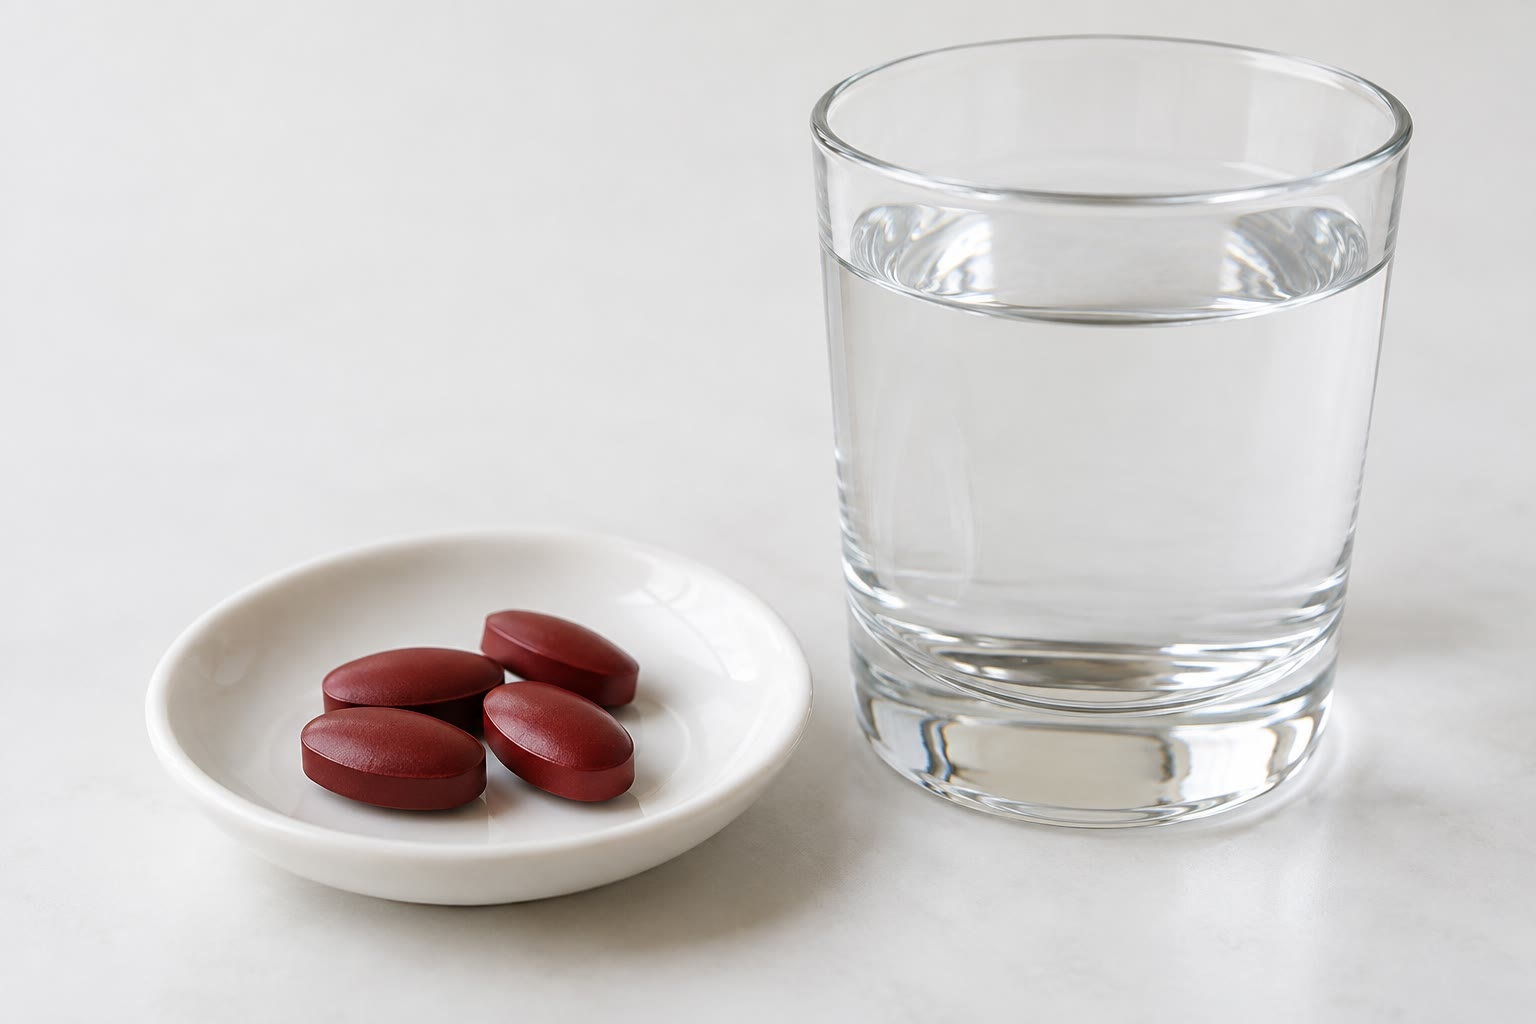
\includegraphics[width=0.45\linewidth]{images/book1/ai/g11-iron-tablets.jpg}

{\small Des comprimés de complément en fer~: combien de fer chacun
contient-il vraiment~?}
\end{omfigure}

\section{Titrer}

\begin{definition}[Titrage, solution titrante, solution titrée]\label{def:g11:titration:titration}
Un \emph{titrage}\index{titrage} mesure la quantité d'une espèce dissoute
en la faisant réagir avec une autre espèce dont la concentration est
connue avec précision. La solution de concentration connue, ajoutée à
l'aide d'une burette, est la \emph{solution titrante}\index{solution titrante}~;
la solution qui contient l'espèce à doser, placée dans l'erlenmeyer, est
la \emph{solution titrée}\index{solution titree@solution titrée}.
\end{definition}

\begin{proposition}[Ce que doit être une réaction de titrage]\label{prop:g11:titration:conditions}
Une réaction peut servir à un \omterm{def:g11:titration:titration}{titrage} si elle est totale (pour qu'un
\omterm{def:g7:chemical-reactions:reactant}{réactif} soit entièrement consommé), rapide (pour que chaque goutte
réagisse aussitôt) et unique (le \omterm{def:g7:chemical-reactions:reactant}{réactif} titrant ne réagit avec rien
d'autre dans l'erlenmeyer).
\end{proposition}

\begin{proof}
Si la réaction s'arrêtait avant d'être complète, prenait du retard sur
les gouttes, ou consommait du \omterm{def:g7:chemical-reactions:reactant}{réactif} titrant ailleurs, le volume versé
ne mesurerait plus la quantité de l'espèce titrée.
\end{proof}

\begin{omfigure}
\begin{tikzpicture}[font=\small, scale=0.62]
  \pic[transform shape] at (0,0) {stand={5.8}{1.8}};
  \pic[transform shape] at (1.8,0.68) {stirrer};
  \pic[transform shape] at (1.8,0.68) {erlenmeyer={0.25}{yellow!12}};
  \pic[transform shape] at (1.8,2.98) {burette={0.75}{violet!55}};
  \draw[omProp, thick, <-] (2.15,6.9) -- (4.2,7.4) node[right, text=black,
    align=left] {burette~: solution titrante\\ (permanganate de potassium)};
  \draw[omProp, thick, <-] (2.55,1.4) -- (4.2,1.9) node[right, text=black,
    align=left] {erlenmeyer~: solution titrée\\ (fer(II), acide)};
  \draw[omProp, thick, <-] (3.0,0.4) -- (4.2,0.3) node[right, text=black]
    {agitateur magnétique};
\end{tikzpicture}

{\small Un montage de \omterm{def:g11:titration:titration}{titrage}~: la burette, tenue par un support, délivre
la \omterm{def:g11:titration:titration}{solution titrante} dans la \omterm{def:g11:titration:titration}{solution titrée}, maintenue sous agitation.}
\end{omfigure}

\section{L'équivalence}

\begin{definition}[Équivalence, volume à l'équivalence]\label{def:g11:titration:equivalence}
L'\emph{équivalence}\index{equivalence@équivalence} est le moment d'un \omterm{def:g11:titration:titration}{titrage} où le
\omterm{def:g7:chemical-reactions:reactant}{réactif} titrant ajouté et l'espèce titrée sont dans les proportions de
l'équation~: tous deux sont entièrement consommés. Le volume de \omterm{def:g11:titration:titration}{solution
titrante} versé à cet instant est le \emph{volume à
l'équivalence}\index{volume a l'equivalence@volume à l'équivalence}, $V_E$.
\end{definition}

\begin{proposition}[La relation à l'équivalence]\label{prop:g11:titration:relation}
Pour une réaction de \omterm{def:g11:titration:titration}{titrage} $a\,\ce{A} + b\,\ce{B} \longrightarrow$
produits, où A est titré (quantité $n_A$) par une \omterm{def:g11:titration:titration}{solution titrante} de B
de concentration $c_B$, on a à l'\omterm{def:g11:titration:equivalence}{équivalence}
\[
  \frac{n_A}{a} = \frac{c_B\, V_E}{b} .
\]
\end{proposition}

\begin{proof}
À l'\omterm{def:g11:titration:equivalence}{équivalence}, le \omterm{def:g6:pure-substances-and-mixtures:mixture}{mélange} est stœchiométrique
(\cref{ch:g10:reaction-progress-table})~: A et B, de quantités initiales
$n_A$ et $c_B V_E$, s'épuisent ensemble, donc $n_A / a = c_B V_E / b$.
\end{proof}

\begin{omfigure}
\begin{tikzpicture}
\begin{axis}[width=0.72\linewidth, height=5.6cm, xmin=0, xmax=20,
    ymin=0, ymax=16, xlabel={volume de solution titrante versé (\si{mL})},
    ylabel={quantité ($\num{e-4}$ \si{mol})}, axis lines*=left, ymajorgrids,
    grid style={gray!20}, tick label style={font=\small},
    label style={font=\small}, legend style={font=\small, at={(0.98,0.97)},
    anchor=north east, draw=none}, legend cell align=left]
  \addplot[very thick, orange!70!black, domain=0:14.3] {14.3 - x};
  \addplot[very thick, violet, domain=14.3:20] {0.2*(x - 14.3)};
  \addplot[very thick, violet, domain=0:14.3, forget plot] {0};
  \legend{\ce{Fe^{2+}} restant dans l'erlenmeyer, \ce{MnO4^-} en excès}
  \addplot[dashed, black!60] coordinates {(14.3,0) (14.3,7)};
  \node[font=\small, anchor=west] at (axis cs:14.5,6.5) {$V_E = \qty{14.3}{mL}$};
\end{axis}
\end{tikzpicture}

{\small Le fer(II) titré par le permanganate à \qty{0.0200}{mol/L}~: les
\omterm{def:g9:ions:ion}{ions} fer(II) s'épuisent exactement au \omterm{def:g11:titration:equivalence}{volume à l'équivalence}~; au-delà,
les \omterm{def:g9:ions:ion}{ions} permanganate ne sont plus consommés et s'accumulent.}
\end{omfigure}

\section{Repérer l'équivalence par un changement de couleur}


\begin{proposition}[Voir l'équivalence]\label{prop:g11:titration:colour}
Quand l'une des espèces du \omterm{def:g11:titration:titration}{titrage} est colorée, l'\omterm{def:g11:titration:equivalence}{équivalence} se voit
par un changement de couleur dans l'erlenmeyer~: la couleur du \omterm{def:g7:chemical-reactions:reactant}{réactif}
titrant apparaît et persiste dès qu'il est en excès, ou la couleur de
l'espèce titrée disparaît quand elle s'épuise.
\end{proposition}

\begin{proof}
Avant l'\omterm{def:g11:titration:equivalence}{équivalence}, chaque \omterm{def:g9:ions:ion}{ion} du \omterm{def:g7:chemical-reactions:reactant}{réactif} titrant qui tombe dans
l'erlenmeyer est aussitôt consommé~; après l'\omterm{def:g11:titration:equivalence}{équivalence}, il subsiste.
Une espèce colorée n'est donc présente dans l'erlenmeyer que d'un seul
côté de l'\omterm{def:g11:titration:equivalence}{équivalence}.
\end{proof}

\begin{example}[Le permanganate, son propre indicateur]\label{ex:g11:titration:permanganate}
L'\omterm{def:g9:ions:ion}{ion} permanganate \ce{MnO4^-} est violet foncé, et les \omterm{def:g9:ions:ion}{ions} manganèse
\ce{Mn^{2+}} qu'il donne sont presque incolores~; les \omterm{def:g9:ions:ion}{ions} fer ne donnent
à la solution qu'une teinte jaune pâle. Avant l'\omterm{def:g11:titration:equivalence}{équivalence}, chaque
goutte violette se décolore en tombant~; la première goutte qui ne se
décolore pas marque l'\omterm{def:g11:titration:equivalence}{équivalence}~: l'erlenmeyer devient rose pâle et le
reste.
\end{example}

\begin{omfigure}
\begin{tikzpicture}[font=\small]
  \pic at (0,0) {erlenmeyer={0.3}{yellow!14}};
  \pic at (3.2,0) {erlenmeyer={0.3}{magenta!10}};
  \pic at (6.4,0) {erlenmeyer={0.3}{violet!45}};
  \node[align=center, anchor=north] at (0,-0.15) {avant l'équivalence~:\\
    jaune pâle, chaque goutte\\ se décolore};
  \node[align=center, anchor=north] at (3.2,-0.15) {à l'équivalence~:\\
    un rose pâle qui\\ persiste};
  \node[align=center, anchor=north] at (6.4,-0.15) {après l'équivalence~:\\
    violet (permanganate\\ en excès)};
\end{tikzpicture}

{\small L'erlenmeyer d'un \omterm{def:g11:titration:titration}{titrage} du fer(II) par le permanganate, avant,
à et après l'\omterm{def:g11:titration:equivalence}{équivalence}. On lit le \omterm{def:g11:titration:equivalence}{volume à l'équivalence} au premier
rose persistant.}
\end{omfigure}

\begin{example}[La vitamine C et le diiode]\label{ex:g11:titration:vitamin-c}
% ledger: aw:C, aw:H, aw:O
La vitamine C, l'acide ascorbique \ce{C6H8O6} ($M = \qty{176.0}{g/mol}$),
est un \omterm{def:g11:redox:oxidant}{réducteur}~; le diiode \ce{I2} l'oxyde~:
\[
  \ce{C6H8O6 + I2 -> C6H6O6 + 2H+ + 2I-} .
\]
On titre \qty{10.0}{mL} de jus d'orange, additionnés d'un peu d'empois
d'amidon, par une solution de diiode à \qty{5.00e-3}{mol/L}. Avant
l'\omterm{def:g11:titration:equivalence}{équivalence}, le diiode est consommé~; la première goutte en excès
colore l'amidon en bleu foncé. Si $V_E = \qty{5.70}{mL}$, le jus
contenait
$n = \num{5.00e-3} \times \num{5.70e-3} = \qty{2.85e-5}{mol}$ de
vitamine C, soit \qty{5.0}{mg} dans \qty{10.0}{mL}~: \qty{0.50}{g/L}.
\end{example}

\section{Calculer une concentration inconnue}

\begin{method}[Calculer une concentration à partir d'un titrage]\label{met:g11:titration:computing}
\begin{enumerate}
  \item Écrire l'\omterm{def:g8:balanced-equations:equation}{équation ajustée} de la réaction de \omterm{def:g11:titration:titration}{titrage} et lire les
        coefficients $a$ (espèce titrée) et $b$ (\omterm{def:g7:chemical-reactions:reactant}{réactif} titrant).
  \item Lire $V_E$ sur la burette, et calculer la quantité de \omterm{def:g7:chemical-reactions:reactant}{réactif}
        titrant versée, $n_B = c_B V_E$.
  \item À l'\omterm{def:g11:titration:equivalence}{équivalence}, $n_A = \dfrac{a}{b}\, c_B V_E$.
  \item Diviser par le volume titré~: $c_A = n_A / V_A$. Si
        l'échantillon a été dilué avant le \omterm{def:g11:titration:titration}{titrage}, multiplier par le
        \omterm{def:g10:concentration-and-dilution:dilution}{facteur de dilution}.
\end{enumerate}
\end{method}

\begin{example}[Une solution de fer(II)]\label{ex:g11:titration:iron}
\qty{20.0}{mL} d'une solution de fer(II), acidifiée, demandent
$V_E = \qty{12.6}{mL}$ de permanganate à \qty{0.0200}{mol/L}. Ici
$a = 5$ (\ce{Fe^{2+}}) et $b = 1$ (\ce{MnO4^-})~:
$n(\ce{MnO4^-}) = 0.0200 \times 0.0126 = \qty{2.52e-4}{mol}$, donc
$n(\ce{Fe^{2+}}) = 5 \times \num{2.52e-4} = \qty{1.26e-3}{mol}$, et
$c(\ce{Fe^{2+}}) = \num{1.26e-3} / 0.0200 = \qty{0.0630}{mol/L}$.
\end{example}

\section{Le titrage, une mesure}

\begin{inthelab}[Lire une burette]
On rince la burette avec la \omterm{def:g11:titration:titration}{solution titrante}, on la remplit, et on
chasse les bulles d'\omterm{def:g4:air-a-mixture-of-gases:air}{air} de sa pointe. On lit le niveau au bas du
ménisque, l'œil à la même hauteur, avant et après le \omterm{def:g11:titration:titration}{titrage}~: le volume
versé est la différence. Les graduations sont tous les \qty{0.1}{mL}, et
une lecture peut être estimée à \qty{0.05}{mL} près. Près de
l'\omterm{def:g11:titration:equivalence}{équivalence}, on ajoute la \omterm{def:g11:titration:titration}{solution titrante} goutte à goutte, en
agitant l'erlenmeyer.
\end{inthelab}

\begin{omfigure}
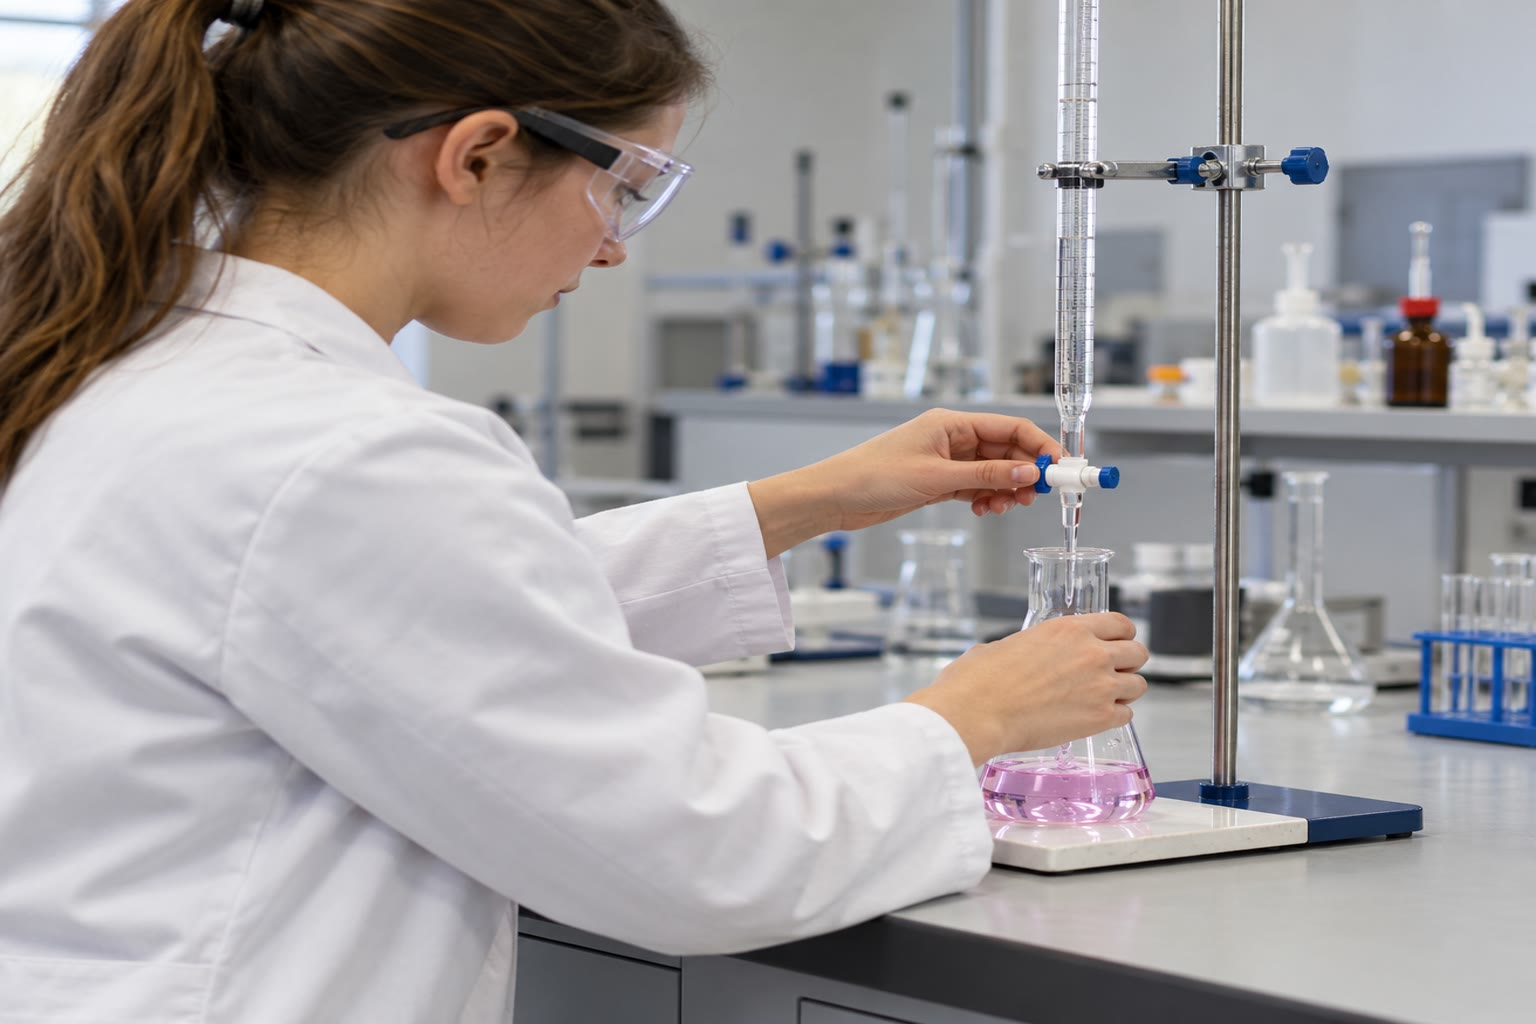
\includegraphics[width=0.48\linewidth]{images/book1/ai/g11-titration-bench.jpg}

{\small Un \omterm{def:g11:titration:titration}{titrage} en cours~: burette, support et erlenmeyer posé sur un
carreau blanc.}
\end{omfigure}

\begin{remark}[Quelle est la précision d'un titrage~?]\label{rem:g11:titration:precision}
Chaque lecture de la burette peut être fausse d'environ \qty{0.05}{mL},
et le volume versé est la différence de deux lectures~: il peut être faux
de \qty{0.1}{mL}. Pour $V_E = \qty{14.3}{mL}$, cela fait $0.1 / 14.3 \approx
\qty{0.7}{\percent}$. Un $V_E$ plus grand diminue cette erreur relative~:
c'est pourquoi on choisit les concentrations des \omterm{def:g11:titration:titration}{solutions titrantes} de
façon à obtenir des \omterm{def:g11:titration:equivalence}{volumes à l'équivalence} de 10 à \qty{20}{mL} avec
une burette de \qty{25}{mL}. On recommence le \omterm{def:g11:titration:titration}{titrage} jusqu'à ce que deux
résultats concordent à \qty{0.1}{mL} près environ. Un traitement plus
fin de l'incertitude d'une mesure est donné dans le volume de première
année d'université.
\end{remark}

\begin{safety}{\ghs[0.7cm]{GHS03}\ghs[0.7cm]{GHS05}\ghs[0.7cm]{GHS07}\ghs[0.7cm]{GHS08}\ghs[0.7cm]{GHS09}}
% ledger: ghs:KMnO4, ghs:I2
Le permanganate de potassium solide est un comburant qui peut
entretenir un incendie, corrosif et nocif~; ses solutions diluées tachent
la peau et les vêtements en brun. Les solutions de diiode sont nocives.
Lunettes et gants~; les déchets sont récupérés, jamais versés dans
l'évier.
\end{safety}

\section{Exercices}


\begin{exercise}[$\star$]\label{exo:g11:titration:1}
Dans un \omterm{def:g11:titration:titration}{titrage}, qu'est-ce que la \omterm{def:g11:titration:titration}{solution titrante}~? La \omterm{def:g11:titration:titration}{solution
titrée}~? Que se passe-t-il à l'\omterm{def:g11:titration:equivalence}{équivalence}~?
\end{exercise}

\begin{exercise}[$\star$]\label{exo:g11:titration:2}
Quelle quantité d'\omterm{def:g9:ions:ion}{ions} permanganate est contenue dans \qty{12.5}{mL}
d'une solution à \qty{0.0200}{mol/L}~?
\end{exercise}

\begin{exercise}[$\star$]\label{exo:g11:titration:3}
Sur la figure des quantités en fonction du volume versé, lire le \omterm{def:g11:titration:equivalence}{volume
à l'équivalence}. Quelle quantité de fer(II) y avait-il dans
l'erlenmeyer au départ~?
\end{exercise}

\begin{exercise}[$\star$]\label{exo:g11:titration:4}
Pourquoi n'a-t-on besoin d'aucun indicateur pour un \omterm{def:g11:titration:titration}{titrage} par le
permanganate~?
\end{exercise}

\begin{exercise}[$\star$]\label{exo:g11:titration:5}
À l'\omterm{def:g11:titration:equivalence}{équivalence} du \omterm{def:g11:titration:titration}{titrage} du fer(II) par le permanganate, quel est le
rapport de la quantité de fer(II) à la quantité de permanganate versée~?
Pourquoi~?
\end{exercise}

\begin{exercise}[$\star\star$]\label{exo:g11:titration:6}
\qty{10.0}{mL} d'une solution acidifiée de fer(II) demandent
\qty{8.40}{mL} de permanganate à \qty{0.0200}{mol/L}. Calculer la
\omterm{def:g10:concentration-and-dilution:molar-concentration}{concentration molaire} en fer(II), puis sa \omterm{def:g10:concentration-and-dilution:mass-concentration}{concentration massique}.
\end{exercise}

\begin{exercise}[$\star\star$]\label{exo:g11:titration:7}
On dissout un comprimé de vitamine C pour obtenir \qty{100.0}{mL} de
solution. \qty{10.0}{mL} de celle-ci, additionnés d'amidon, demandent
\qty{11.4}{mL} de diiode à \qty{0.0100}{mol/L}. Quelle masse de
vitamine C le comprimé contient-il~?
\end{exercise}

\begin{exercise}[$\star\star$]\label{exo:g11:titration:8}
Une réaction est totale mais dure plusieurs minutes. Pourquoi ne
peut-elle pas servir telle quelle à un \omterm{def:g11:titration:titration}{titrage} avec changement de
couleur~?
\end{exercise}

\begin{exercise}[$\star\star$]\label{exo:g11:titration:9}
Observer les trois erlenmeyers. Une élève s'arrête à un erlenmeyer aussi
violet que le troisième. Son \omterm{def:g11:titration:equivalence}{volume à l'équivalence} est-il trop grand ou
trop petit~? Qu'aurait-elle dû faire près de l'\omterm{def:g11:titration:equivalence}{équivalence}~?
\end{exercise}

\begin{exercise}[$\star\star$]\label{exo:g11:titration:10}
Une solution concentrée de fer(II) est d'abord diluée dix fois. Puis
\qty{10.0}{mL} de la solution diluée demandent \qty{13.0}{mL} de
permanganate à \qty{0.0200}{mol/L}. Déterminer la concentration de la
solution concentrée.
\end{exercise}

\begin{exercise}[$\star\star$]\label{exo:g11:titration:11}
% ledger: aw:Fe
La solution de fer(II) de l'exemple traité dans le chapitre a pour
concentration $c = \qty{0.0630}{mol/L}$. Quelle masse de fer
\qty{1.00}{L} de cette solution contient-il~?
\end{exercise}

\begin{exercise}[$\star\star\star$]\label{exo:g11:titration:12}
Un \omterm{def:g11:titration:titration}{titrage} donne $V_E = \qty{7.2}{mL}$. Estimer l'erreur relative due
aux lectures de la burette, et la comparer à celle obtenue pour
$V_E = \qty{14.3}{mL}$. Proposer deux moyens d'obtenir un \omterm{def:g11:titration:equivalence}{volume à
l'équivalence} plus grand.
\end{exercise}

\begin{exercise}[$\star\star\star$]\label{exo:g11:titration:13}
On titre le peroxyde d'hydrogène par le permanganate en milieu acide~:
\[
  \ce{2MnO4^- + 5H2O2 + 6H+ -> 2Mn^{2+} + 5O2 + 8H2O} .
\]
On dilue dix fois un désinfectant~; \qty{10.0}{mL} de la solution diluée
demandent \qty{17.6}{mL} de permanganate à \qty{0.0200}{mol/L}.
Déterminer la \omterm{def:g10:concentration-and-dilution:molar-concentration}{concentration molaire} du peroxyde d'hydrogène dans le
désinfectant, puis sa \omterm{def:g10:concentration-and-dilution:mass-concentration}{concentration massique} (\ce{H2O2}~:
\qty{34.0}{g/mol}).
\end{exercise}

\begin{exercise}[$\star\star\star$]\label{exo:g11:titration:14}
Un comprimé de fer doit contenir environ \qty{1.4e-3}{mol} de fer(II).
Quelle concentration de permanganate donne un \omterm{def:g11:titration:equivalence}{volume à l'équivalence}
voisin de \qty{15}{mL} avec une burette de \qty{25}{mL}~? Qu'est-ce qui
n'irait pas avec une solution dix fois plus concentrée~?
\end{exercise}

\begin{exercise}[$\star\star\star$]\label{exo:g11:titration:15}
L'équation du \omterm{def:g11:titration:titration}{titrage} comporte \ce{8H+} pour chaque \ce{MnO4^-}. Pour un
\omterm{def:g11:titration:equivalence}{volume à l'équivalence} de \qty{14.3}{mL} à \qty{0.0200}{mol/L}, quelle
quantité d'\omterm{def:g9:ions:ion}{ions} hydrogène est consommée~? \qty{10}{mL} d'un acide
contenant \qty{1.0}{mol/L} d'\omterm{def:g9:ions:ion}{ions} hydrogène suffisent-ils~? Pourquoi
faut-il acidifier l'erlenmeyer~?
\end{exercise}

\section{Problème~: le comprimé de fer est-il honnête~?}

\begin{problem}[{Problème du week-end --- un complément en fer annonce
80~mg de fer par comprimé~: un titrage le confirme-t-il~?}]
\label{pb:g11:titration:1}
% ledger: aw:Fe, aw:S, aw:O, const:NA
La boîte d'un complément en fer annonce \qty{80}{mg} de fer, sous forme
de fer(II), par comprimé. On broie un comprimé et on le dissout dans
environ \qty{50}{mL} d'acide sulfurique dilué, puis on le titre par du
permanganate de potassium à \qty{0.0200}{mol/L}. Le rose pâle persiste
pour $V_E = \qty{14.3}{mL}$.

\medskip
\noindent\textbf{Partie I --- La réaction.}
\begin{enumerate}
  \item Nommer les deux \omterm{def:g11:redox:couple}{couples oxydant/réducteur} mis en jeu. Quelle
        espèce est l'\omterm{def:g11:redox:oxidant}{oxydant}, laquelle le \omterm{def:g11:redox:oxidant}{réducteur}~?
  \item Écrire les deux \omterm{def:g11:redox:couple}{demi-équations}.
  \item Les combiner pour obtenir l'équation du \omterm{def:g11:titration:titration}{titrage}, et vérifier
        qu'elle est ajustée en charges.
  \item Pourquoi dissout-on le comprimé dans un acide~?
  \item Montrer que la réaction remplit les conditions d'un \omterm{def:g11:titration:titration}{titrage}, et
        expliquer comment on voit l'\omterm{def:g11:titration:equivalence}{équivalence}.
\end{enumerate}

\medskip
\noindent\textbf{Partie II --- Le \omterm{def:g11:titration:titration}{titrage}.}
\begin{enumerate}[resume]
  \item Dans quelle pièce de verrerie se trouve la solution de
        permanganate~? Comment lit-on son volume~?
  \item De quelle couleur est l'erlenmeyer avant l'\omterm{def:g11:titration:equivalence}{équivalence}, et
        pourquoi chaque goutte se décolore-t-elle~?
  \item Calculer la quantité de permanganate versée à l'\omterm{def:g11:titration:equivalence}{équivalence}.
\end{enumerate}

\medskip
\noindent\textbf{Partie III --- Le fer.}
\begin{enumerate}[resume]
  \item En déduire la quantité de fer(II) dans le comprimé.
  \item Calculer sa masse en milligrammes.
  \item Comparer avec l'étiquette~: quel écart relatif~?
  \item Le volume versé peut être faux de \qty{0.1}{mL}. De combien de
        milligrammes la masse de fer peut-elle être fausse~? L'étiquette
        est-elle confirmée~?
\end{enumerate}

\medskip
\noindent\textbf{Partie IV --- Plusieurs comprimés.}
\begin{enumerate}[resume]
  \item Deux autres comprimés donnent $V_E = \qty{14.1}{mL}$ et
        \qty{14.4}{mL}. Calculer leurs masses de fer.
  \item Calculer la moyenne des trois comprimés.
  \item Les trois résultats diffèrent de plus que l'erreur de la
        burette. Que cela indique-t-il sur les comprimés~?
  \item Du permanganate à \qty{0.100}{mol/L} aurait-il été un meilleur
        choix~? Expliquer.
  \item Beaucoup de compléments contiennent aussi de la vitamine C, un
        \omterm{def:g11:redox:oxidant}{réducteur}. Quel effet aurait-elle sur le \omterm{def:g11:titration:titration}{titrage}, et sur la masse
        de fer trouvée~?
  \item Le fer est présent sous forme de sulfate de fer(II), \ce{FeSO4}.
        Quelle masse de ce composé un comprimé contient-il~?
  \item Combien d'\omterm{def:g9:ions:ion}{ions} fer(II) cela représente-t-il~?
  \item Donner la réponse finale~: quelle masse de fer un comprimé
        contient-il~?
\end{enumerate}
\end{problem}
